\RequirePackage{currfile}
\documentclass[12pt]{beamer}
\usepackage[utf8]{inputenc}
\usepackage[spanish]{babel}
\usepackage{standalone}
\usepackage{color}
\usepackage{siunitx}
\usepackage{hyperref}
%\hypersetup{colorlinks,linkcolor=,urlcolor=blue}
%\hypersetup{colorlinks,urlcolor=blue}
\usepackage{xcolor,soul}
\usepackage{etoolbox}
\usepackage{amsmath}
\usepackage{amsthm}
\usepackage{physics}
\usepackage{multicol}
\usepackage{bookmark}
\usepackage{longtable}
\usepackage{listings}
\usepackage{graphicx}
\usepackage{tikz}
\usetikzlibrary{patterns, matrix, backgrounds, decorations,shapes, arrows.meta}
\usepackage[autostyle,spanish=mexican]{csquotes}
\usepackage[os=win]{menukeys}
\usepackage{pifont}
\usepackage{pbox}
\usepackage{caption}
\captionsetup{font=scriptsize,labelfont=scriptsize}
%\usepackage[sfdefault]{roboto}  %% Option 'sfdefault' only if the base font of the document is to be sans serif

%Sección de definición de colores
\definecolor{ao}{rgb}{0.0, 0.5, 0.0}
\definecolor{bisque}{rgb}{1.0, 0.89, 0.77}
\definecolor{amber}{rgb}{1.0, 0.75, 0.0}
\definecolor{armygreen}{rgb}{0.29, 0.33, 0.13}
\definecolor{alizarin}{rgb}{0.82, 0.1, 0.26}
\definecolor{cadetblue}{rgb}{0.37, 0.62, 0.63}
\definecolor{deepblue}{rgb}{0,0,0.5}
\definecolor{brown}{rgb}{0.59, 0.29, 0.0}
\definecolor{OliveGreen}{rgb}{0,0.25,0}


\usefonttheme[onlymath]{serif}
%Sección de definición de nuevos comandos

\newcommand*{\TitleParbox}[1]{\parbox[c]{1.75cm}{\raggedright #1}}%
\newcommand{\python}{\texttt{python}}
\newcommand{\textoazul}[1]{\textcolor{blue}{#1}}
\newcommand{\azulfuerte}[1]{\textcolor{blue}{\textbf{#1}}}
\newcommand{\funcionazul}[1]{\textcolor{blue}{\textbf{\texttt{#1}}}}
\newcommand{\ptilde}[1]{\ensuremath{{#1}^{\prime}}}
\newcommand{\stilde}[1]{\ensuremath{{#1}^{\prime \prime}}}
\newcommand{\ttilde}[1]{\ensuremath{{#1}^{\prime \prime \prime}}}
\newcommand{\ntilde}[2]{\ensuremath{{#1}^{(#2)}}}
\renewcommand{\arraystretch}{1.5}

\newcounter{saveenumi}
\newcommand{\seti}{\setcounter{saveenumi}{\value{enumi}}}
\newcommand{\conti}{\setcounter{enumi}{\value{saveenumi}}}
\renewcommand{\rmdefault}{cmr}% cmr = Computer Modern Roman

\linespread{1.5}

\usefonttheme{professionalfonts}
%\usefonttheme{serif}
\DeclareGraphicsExtensions{.pdf,.png,.jpg}


%Sección para el tema de beamer, con el theme, usercolortheme y sección de footers
\mode<presentation>
{
  \usetheme{Warsaw}
  
  %\useoutertheme{infolines}
  \useoutertheme{default}
  \usecolortheme{spruce}
  \setbeamercovered{invisible}
  % or whatever (possibly just delete it)
  \setbeamertemplate{section in toc}[sections numbered]
  \setbeamertemplate{subsection in toc}[subsections numbered]
  \setbeamertemplate{subsection in toc}{\leavevmode\leftskip=3.2em\rlap{\hskip-2em\inserttocsectionnumber.\inserttocsubsectionnumber}\inserttocsubsection\par}
  \setbeamercolor{section in toc}{fg=blue}
  \setbeamercolor{subsection in toc}{fg=blue}
  \setbeamercolor{frametitle}{fg=blue}
  \setbeamertemplate{caption}[numbered]

  \setbeamertemplate{footline}
  \beamertemplatenavigationsymbolsempty
  \setbeamertemplate{headline}{}
}

\makeatletter
\setbeamercolor{section in foot}{bg=gray!30, fg=black!90!orange}
\setbeamercolor{subsection in foot}{bg=blue!30!yellow, fg=red}
\setbeamertemplate{footline}
{
  \leavevmode%
  \hbox{%
  \begin{beamercolorbox}[wd=.333333\paperwidth,ht=2.25ex,dp=1ex,center]{section in foot}%
    \usebeamerfont{section in foot} \insertsection
  \end{beamercolorbox}}%
  \begin{beamercolorbox}[wd=.333333\paperwidth,ht=2.25ex,dp=1ex,center]{subsection in foot}%
    \usebeamerfont{subsection in foot}  \insertsubsection
  \end{beamercolorbox}%
  \begin{beamercolorbox}[wd=.333333\paperwidth,ht=2.25ex,dp=1ex,right]{date in head/foot}%
    \usebeamerfont{date in head/foot} \insertshortdate{} \hspace*{2em}
    \insertframenumber{} / \inserttotalframenumber \hspace*{2ex} 
  \end{beamercolorbox}}%
  \vskip0pt%
\makeatother  

\makeatletter
\patchcmd{\beamer@sectionintoc}
  {\vfill}
  {\vskip\itemsep}
  {}
  {}
\makeatother


\title{\large{Objetivos del Tema 1 - La física y la geometría}}
\subtitle{Curso MAF}
\author{M. en C. Gustavo Contreras Mayén}
\date{\today}
\institute{Facultad de Ciencias - UNAM}
\titlegraphic{
\includegraphics[width=1.75cm]{../Imagenes/escudo-facultad-ciencias}\hspace*{4.75cm}~%
   
\includegraphics[width=1.75cm]{../Imagenes/escudo-unam}
}
\setbeamertemplate{navigation symbols}{}
\begin{document}
\maketitle
\fontsize{14}{14}\selectfont
\spanishdecimal{.}
\section*{Contenido}
\frame[allowframebreaks]{\tableofcontents[currentsection, hideallsubsections]}
\section{Introducción}
\frame[allowframebreaks]{\tableofcontents[currentsection, hideothersubsections]}
\subsection{Sistemas conocidos}
\begin{frame}
\frametitle{Introducción}
Estamos familiarizados con el uso de distintos sistemas coordenados para describir problemas físicos.
\\
\bigskip
Hemos usado coordenadas cartesianas, cilíndricas y esféricas para problemas con esas simetrías.
\end{frame}
\begin{frame}
\frametitle{Otros sistemas}
Veremos que existen otros sistemas coordenados que poco a poco durante la carrera, nos encontraremos con ellos para problemas en particular.
\\
\bigskip
\pause
El Tema 1 nos brindará una estrategia de trabajo con ellos.
\end{frame}
\section{Ejemplos}
\frame{\tableofcontents[currentsection, hideothersubsections]}
\subsection{Dos ejemplos}
\begin{frame}
\frametitle{Ejemplo}
Consideremos el vector campo eléctrico $(\vb{E})$ creado por una carga puntual $q$ localizada en el origen de un sistema cartesiano. Usando los vectores de la base, el campo es:
\begin{align*}
\va{\vb{E}} = \dfrac{q}{4 \pi \varepsilon_{0}} \, \dfrac{x \, \vu{e}_{x} + y \, \vu{e}_{y} + z \, \vu{e}_{z}}{\left( x^{2} + y^{2} + z^{2} \right)^{3/2}}
\end{align*}
\end{frame}
\begin{frame}
\frametitle{Ejemplo}
En coordenadas esféricas $(r, \theta, \phi)$, en donde se aprovecha completamente la simetría del problema para este campo, se simplifica la expresión anterior, así el campo eléctrico resulta ser:
\begin{align*}
\va{\vb{E}} = \dfrac{q}{4 \pi \varepsilon_{0}} \, \dfrac{\vu{e}_{r}}{r^{2}}
\end{align*}
\end{frame}
\begin{frame}
\frametitle{Otro ejemplo}
Ahora consideramos un problema con ondas estacionarias en un sistema bidimensional con simetría circular: la de una membrana circular delgada y perfectamente flexible (por ejemplo, una membrana de tambor circular idealizada) de radio $r$,
\end{frame}
\begin{frame}
\frametitle{Otro ejemplo}
La ecuación de onda en coordenadas bidimensionales cilíndricas $(x , y \rightarrow r, \varphi)$ para la amplitud de desplazamiento, $\psi (r, \varphi, t)$ viene dada por:
\begin{align*}
\laplacian \psi (r, \varphi, t) - \dfrac{1}{v^{2}} \pdv[2]{\psi (r, \varphi, t)}{t} = 0
\end{align*}
\end{frame}
\begin{frame}
\frametitle{Elegir el sistema coordenado}
Para la elección del sistema coordenado debemos de considerar aquel en donde la simetría del problema nos simplique el trabajo.
\\
\bigskip
\pause
En este caso, corresponde elegir el sistema coordenado cilíndrico.
\end{frame}
\begin{frame}
\frametitle{Reexpresar la ecuación de onda}
Una vez elegido el sistema coordenado, debemos de realizar lo necesario para reexpresar la ecuación diferencial del problema en el sistema.
\\
\bigskip
\pause
Habrá que \enquote{adaptar} el operador Laplaciano en este sistema.
\end{frame}
\begin{frame}
\frametitle{Solución a la ED obtenida}
Una vez que se realiza la reexpresión de la ED, el siguiente paso es resolverla.
\\
\bigskip
\pause
Para ello, ocuparemos lo que se revisará en el \emph{\textcolor{blue}{Primeras técnicas de solución}}.
\end{frame}
\begin{frame}
\frametitle{Solución al problema}
Cuando veamos el tema de \emph{función de Bessel}, tomaremos de nuevo este ejercicio.
\\
\bigskip
\pause
La solución obtenida la podemos ocupar con otras herramientas computacionales para \emph{simular} el comportamiento de la membrana circular.
\end{frame}
\begin{frame}
\frametitle{Solución gráfica}
\begin{figure}[h!]
    \centering
    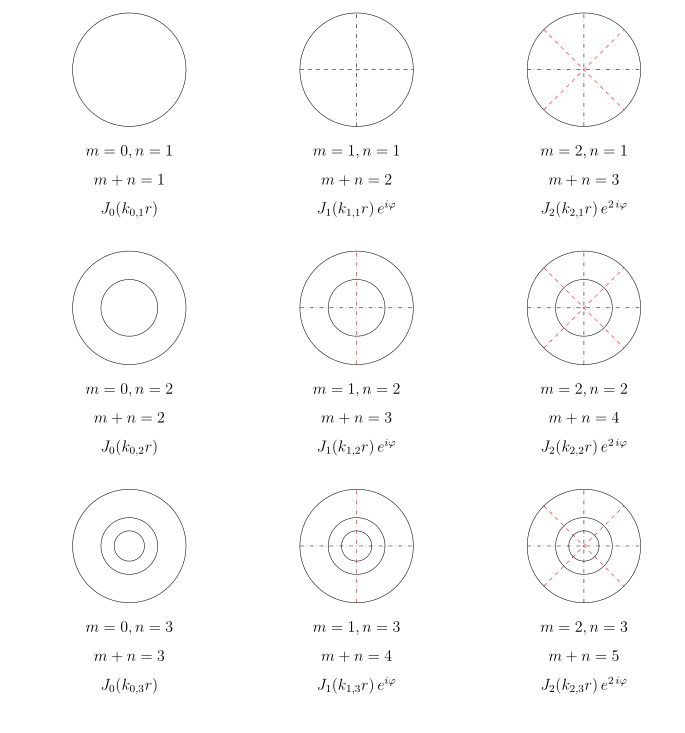
\includegraphics[scale=0.35]{Imagenes/Modos_Vibracion.png}
\end{figure}
\end{frame}
\begin{frame}
\frametitle{Simulación computacional}
\begin{figure}[h!]
    \centering
    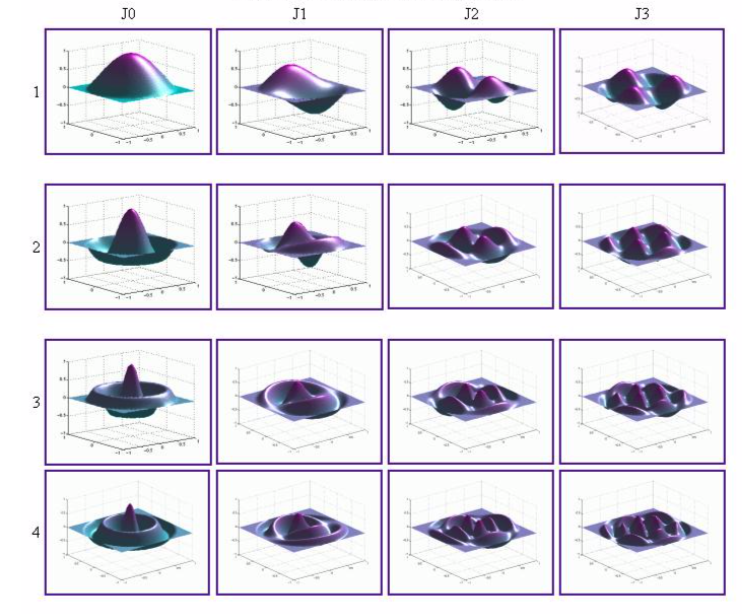
\includegraphics[scale=0.32]{Imagenes/Modos_Normales_Membrana_Circular.png}
\end{figure}
\end{frame}
\section{Objetivos}
\frame{\tableofcontents[currentsection, hideothersubsections]}
\subsection{Tema 1}
\begin{frame}
\frametitle{Objetivos}
Al concluir el Tema 1, el alumno:
\setbeamercolor{item projected}{bg=blue!70!black,fg=yellow}
\setbeamertemplate{enumerate items}[circle]
\begin{enumerate}[<+->]
\item Describirá las superficies coordenadas a partir de las reglas de transformación entre el sistema cartesiano y otro sistema de estudio.
\item Determinará los factores de escala del nuevo sistema de estudio, así como los vectores base y la interpretación con los vectores cartesianos.
\seti
\end{enumerate}
\end{frame}
\begin{frame}
\frametitle{Objetivos}
\setbeamercolor{item projected}{bg=blue!70!black,fg=yellow}
\setbeamertemplate{enumerate items}[circle]
\begin{enumerate}[<+->]
\conti
\item Calculará los operadores diferenciales en el nuevo sistema de estudio.
\item Resolverá mediante las funciones Gamma y Beta ejercicios de la física.
\end{enumerate}
\end{frame}
\section{Trabajo asíncrono}
\frame{\tableofcontents[currentsection, hideothersubsections]}
\subsection{Presentaciones}
\begin{frame}
\frametitle{Trabajo a realizar}
Como se revisó en la presentación del curso de MAF, el trabajo asíncrono por parte del alumno, consistirá en leer los materiales del curso en la plataforma Moodle, siendo los siguientes:
\end{frame}
\begin{frame}
\frametitle{Materiales de trabajo}
\setbeamercolor{item projected}{bg=blue!70!black,fg=yellow}
\setbeamertemplate{enumerate items}[circle]
\begin{enumerate}[<+->]
\item Sistema de coordenadas curvilíneas ortogonales.
\item Diferenciales y operadores diferenciales.
\item Construcción de sistemas coordenados especiales.
\item Funciones Gamma y Beta.
\end{enumerate}
\end{frame}
\begin{frame}
\frametitle{Trabajo por semana}
Recomendamos que la revisión de las presentaciones 1, 2, 3: se realicen durante las semanas 1 y 2.
\\
\bigskip
Para la semana 3, deberán de atender la presentación correspondiente a las funciones Gamma y Beta.
\end{frame}
\begin{frame}
\frametitle{Envío de ejercicios a cuenta}
Considerando que en la semana 1, tendrían 2 días hábiles para la revisión de los materiales, en esta ocasión, los ejercicios resueltos de las presentaciones 1, 2 y 3, deberán de enviarlos a la plataforma el día 16 de octubre.
\end{frame}
\begin{frame}
\frametitle{Envío de ejercicios a cuenta}
Las soluciones a los ejercicios de la semana 3, se enviarán el día 23 de octubre mediante la plataforma.
\end{frame}
\begin{frame}
\frametitle{Materiales complementarios}
Tendrán disponibles materiales complementarios, que como mencionamos en la presentación del curso, les serán de utilidad ya que cuentan con un enfoque elevado, pero lo necesario para una consulta.
\\
\bigskip
Siendo también un atractivo para que extiendan la consulta en las referencias bibliográficas del curso.
\end{frame}
\end{document}